\documentclass[12pt]{article}
\usepackage[top=1in, bottom=1in, left=1in, right=1in]{geometry}

\usepackage{setspace}
\onehalfspacing

\usepackage{amssymb}
%% The amsthm package provides extended theorem environments
\usepackage{amsthm}
\usepackage{epsfig}
\usepackage{times}
\renewcommand{\ttdefault}{cmtt}
\usepackage{amsmath}
\usepackage{graphicx} % for graphics files
\usepackage{tabu}

% Draw figures yourself
\usepackage{tikz} 

% writing elements
\usepackage{mhchem}

% The float package HAS to load before hyperref
\usepackage{float} % for psuedocode formatting
\usepackage{xspace}

% from Denovo Methods Manual
\usepackage{mathrsfs}
\usepackage[mathcal]{euscript}
\usepackage{color}
\usepackage{array}

\usepackage[pdftex]{hyperref}
\usepackage[parfill]{parskip}

% math syntax
\newcommand{\nth}{n\ensuremath{^{\text{th}}} }
\newcommand{\ve}[1]{\ensuremath{\mathbf{#1}}}
\newcommand{\Macro}{\ensuremath{\Sigma}}
\newcommand{\rvec}{\ensuremath{\vec{r}}}
\newcommand{\vecr}{\ensuremath{\vec{r}}}
\newcommand{\omvec}{\ensuremath{\hat{\Omega}}}
\newcommand{\vOmega}{\ensuremath{\hat{\Omega}}}
\newcommand{\sigs}{\ensuremath{\Sigma_s(\rvec,E'\rightarrow E,\omvec'\rightarrow\omvec)}}
\newcommand{\el}{\ensuremath{\ell}}
\newcommand{\sigso}{\ensuremath{\Sigma_{s,0}}}
\newcommand{\sigsi}{\ensuremath{\Sigma_{s,1}}}
%---------------------------------------------------------------------------
%---------------------------------------------------------------------------
\begin{document}
\begin{center}
{\bf NE 250, F15\\
October 26, 2015 
}
\end{center}

Last time we talked about the general algorithm for Monte Carlo for neutral particle transport. \\
We went briefly over probability distributions: PDFs and CDFs. \\
Next up we will go through the very basics of the ideas about sampling, scoring, and statistics.

-------------------------------------------------------\\
\textbf{Sampling}\\
Random sampling uses \underline{uniformly distributed random variables} ($\xi$ distributed between 0 and 1) to choose a value for a variable according to its probability density function.\\
Functionally, you can think of this as doing
\[
F(x) = \xi \quad \rightarrow \quad x = F^{-1}(\xi)\:.
\]
The trick is executing $F^{-1}$, which we cannot always do directly.\\
This gives rise to the need for a variety of sampling techniques (none of which we will really go into).\\
%
\textit{Basic} sampling techniques:
      \begin{itemize}
      \item Direct discrete sampling (which reaction)
      \item Direct continuous sampling (\# mfps)
      \item Rejection sampling (for sampling non-invertible functions like Klien-Nishina)
      \end{itemize}
\textit{Advanced }sampling techniques:
      \begin{itemize}
      \item Histogram
      \item Piecewise linear
      \item Alias sampling
      \item Advanced continuous PDFs
      \end{itemize}
%
The classic example of sampling in MC is the distance between collisions (which is a case where we can do direct inversion).
\begin{itemize}
\item $\Sigma_t$ = total macroscopic cross section of material
\[\Sigma_T = \sum_{j=1}^J N_j \sigma_t^j\]
%
\item The PDF for distance to collision is probability of interaction per unit distance $\times$ probability of traveling distance $s$ without interacting
\[f(s) = \Sigma_t \exp\bigl(-\Sigma_t s \bigr)\]
%
\item We integrate and normalize to get the CDF
\[F(s) = 1 - \exp\bigl(-\Sigma_t s \bigr)\]
%
\item To actually sample this, we invert it and get a random number (also noting that $\ln(1-\xi)$ is distributed the same exact way as $\ln(\xi)$ but the latter requires fewer operations:
\[
s = \frac{-\ln(\xi)}{\Sigma_t}
\]
\end{itemize}
%
If we're in a multi-region problem, we figure out if we intersect a boundary and if so move the particle to that boundary and determine how much farther it goes into the next material before having a collision.

After finding the location of the collision and the isotope collided with, we need to determine \textbf{what type of collision} occurs. 
%
\begin{itemize}
\item $\Sigma_t = \Sigma_{elastic} + \Sigma_{inelastic} + \Sigma_{capture} + \Sigma_{fission} + \dots$.
%
\item The probability of reaction of type $i$ for a given isotope is 
\[p_i = \frac{\Sigma_i}{\Sigma_t}\]
%
\item This gives a set of discrete probabilities, which we can sample 
\begin{itemize}
\item directly: generate $\xi$, determine $k$ s.t. $F_{k-1} \leq \xi \le F_k$, return $i = i_k$.
%
\item or by making an alias table and sampling.
\end{itemize}
\end{itemize}

We use sampling to figure out what happens at every single step of the transport algorithm we talked about last time.\\
Eventually, we also want to record an answer. That's where scoring comes in.

\vspace*{1 em}
-------------------------------------------------------\\
\textbf{Scoring}\\
All we have so far is a collection of histories.\\
Each history, $i$, is just a series of interaction sites.\\
\textit{Estimators} convert each history into a score, $x_i$. \\
Each history has a different score (in general).\\
A \textit{tally} accumulates a set of scores, $\{x_i\}$, to form a probability density function.

Usually we're interested in the \textit{expected value} of the underlying PDF. \\
Tallies are \textit{normalized} to the number of source particles. Thus
\[
E(x) = \frac{1}{N} \sum_{i=1}^N x_i
\]
where $N$ is the number of MC particles in the simulation source.\\
The absolute physical quantities require multiplication by the physical source strength (check for a given Monte Carlo code to ensure this is the way it works). 

%We can choose to subdivide phase space into domains or bins (energy bins for spectra, cosine bins for angular distributions, etc.).

We have three main types of estimators
\begin{enumerate}
\item point estimators: surface crossings (current tally, surface flux tally) and collisions (eigenvalue tally)
\item track length estimator: path length through a cell (volume flux tally)
\item energy balance estimator: energy loss in cell (pulse height tally)
\end{enumerate}
%
I will present the estimator scores with a weight value that scales its contribution to the tally.\\
For now the weight will always be $1$, so you can functionally ignore it. \\

For a surface or current tally, we count particle crossing a surface:
\[
x_i = \sum_j w_{ij} \quad \text{summing over each crossing }j\text{ of history }i
\]
The current is
\[
\int_A dA \int_t dt \int_{\vOmega} d\vOmega \int_E dE\: \hat{n} \cdot \vec{J}(\rvec, E, t) \approx \frac{1}{N} \sum_{i=1}^N x_i = \frac{1}{N} \sum_{i=1}\sum_{i=j} w_{ij}
\]
And the surface energy current is
\[
\int_A dA \int_t dt  \int_{\vOmega} d\vOmega \int_E dE\: E\hat{n} \cdot \vec{J}(\rvec, E) \approx \frac{1}{N} \sum_{i=1}\sum_{i=j} E_{ij}w_{ij}
\]

To get the flux/fluence in a volume
\[
\bar{\phi_V} = \frac{1}{V}\int_V dV \int_t dt \int_E dE\: \phi(\rvec, E,t) =  \frac{1}{V}\int_V dV \int_s ds \int_E dE\: N(\rvec, E,t)
\]
where we noted that $\phi \equiv vN$ and then $vdt = ds$.\\
We can now see that we can use either a collision or a track length estimator for flux.\\
Collision (score happens at collision of particle $i$):
\[
\bar{\phi_V} \approx \frac{1}{V}\frac{1}{N} \sum_{i=1} x_i = \frac{1}{V}\frac{1}{N} \sum_{i=1} w_i
\]
Track length ($N(\rvec, E,t)ds$ is density of track lengths, $T_l$):
\[
\bar{\phi_V} \approx \frac{1}{V}\frac{1}{N} \sum_{i=1}\sum_{i=j} w_{ij}T_{l,ij}
\]

Surface flux can also be obtained with track length tallies by accounting for angle of crossing, $\theta$ and $\mu_{ij} = \cos(\theta_{ij})$. Assume we're thinking of a volume cell that becomes infinitely thin with thickness $\delta$. 
\begin{align*}
T_{l,ij} &= \frac{\delta}{|\cos(\theta_{ij})|}\\
\bar{\phi_A} &\approx \frac{1}{V}\frac{1}{N} \sum_{i=1}\sum_{i=j} w_{ij}\frac{\delta}{|\mu_{ij}|} = \frac{1}{A \delta}\frac{1}{N} \delta \sum_{i=1}\sum_{i=j} \frac{w_{ij}}{|\mu_{ij}|}
\end{align*}
%
And so on for other items of interest.


\clearpage
%-------------------------------------------------------
-------------------------------------------------------\\
\textbf{Statistics}\\
The ``true" mean value, $\mu$, of any PDF is the expected value, $E(x)$
\[
\mu = E(x) = \int x f(x) dx
\]
Because we can't usually do this, we use random samples and estimate the true mean from the ``sample" mean, $\bar{x}$
\[
\bar{x} = \frac{1}{N}\sum_{i=1}^N x_i \qquad \lim_{N \to \infty} \bar{x} \rightarrow \mu\:.
\]
The variance of a PDF is the measure of spread in that PDF
\begin{align*}
\sigma^2 &= E[(x - \mu)^2] = \int (x - \mu)^2 f(x) dx \\
&= \int x^2 f(x) dx - 2 \mu \int x f(x) dx + \mu^2 \int f(x) dx\\
&= E(x^2) - \mu^2
\end{align*}
%
However, we don't know the PDF so we use the samples to get the sample variances
\begin{align*}
S_x^2 &= \frac{1}{N-1}\sum_{i=1}^N (x_i - \bar{x})^2 \\
&= \frac{1}{N-1} \biggl[\sum_{i=1}^N x_i^2 - 2 \bar{x}\sum_{i=1}^N x_i + \bar{x}^2 \sum_{i=1}^N 1 \biggr] \\
&\approx \bar{x^2} - \bar{x}^2
\end{align*}

The \underline{Central Limit Theorem} states that
For $N$ \textit{independent} random variables, $x_i$, sampled from \textit{identical distributions}, their mean follows a Normal (Gaussian) distribution.\\
(Note: this is the \textit{IID} requirement for MC)\\
We can use this information to define \textit{confidence intervals}
\begin{align*}
\bar{x} - S_{\bar{x}} &< E(x) < \bar{x} + S_{\bar{x}} \quad \text{about 68\% of the time}\\
\bar{x} - 2S_{\bar{x}} &< E(x) < \bar{x} + 2S_{\bar{x}} \quad \text{about 95\% of the time}
\end{align*}

The \textbf{standard deviation} of the mean is a measure of the error in the result
\begin{align*}
S_{\bar{x}}^2 &= E[(\bar{x} - \mu)^2] = E\biggl[ \biggl(\frac{1}{N}\sum_{i=1}^N x_i - \mu\biggr)^2\biggr] = E\biggl[ \biggl(\frac{1}{N^2}\sum_{i=1}^N (x_i - \mu)\biggr)^2\biggr]\\
%
&=\frac{1}{N^2} E\biggl[ \sum_{i=1}^N (x_i - \mu) \sum_{j=1}^N (x_j - \mu)\biggr] = \frac{1}{N^2} E\biggl[ \sum_{i=1}^N \sum_{j=1}^N (x_i - \mu)  (x_j - \mu)\biggr]\\
%
&= \frac{1}{N^2} \sum_{i=1}^N \sum_{j=1}^N E\bigl[  (x_i - \mu)  (x_j - \mu)\bigr] = \frac{1}{N^2} \sum_{i=1}^N \sum_{j=1}^N S^2_x \delta_{ij} = \frac{1}{N^2} \sum_{i=1}^N S_x^2 \\
%
&= \frac{N S_x^2}{N^2} = \boxed{\frac{S_x^2}{N}}
\end{align*}
The error in the results decreases with the square of increasing the number of histories.
%
\begin{figure}[h!]
\begin{center}
  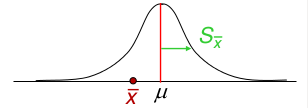
\includegraphics[height=1 in,clip]{../figs/gaussian}
\end{center}
  %\caption{Monte Carlo neutral particle transport algorithm}
  \label{fig:gaussian}
\end{figure}

\textbf{Relative Error} is 
\[
R = \frac{S_{\bar{x}}}{\bar{x}} = \sqrt{\frac{\sum_{i=1}^N x_i^2}{\bigl(\sum_{i=1}^N x_i\bigr)^2} - \frac{1}{N}} 
\]
If $x_i$ are equal and non-zero, R=0.\\
Thus, we can reduce the error by reducing the spread in $x_i$.

\textbf{Accuracy vs.\ Precision}\\
The distinction between accuracy and precision can be seen in Fig.~\ref{fig:accuracy}.\\
%
\begin{figure}[h!]
\begin{center}
  %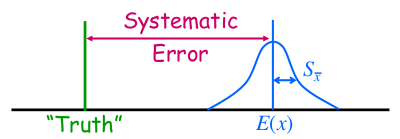
\includegraphics[height=1 in,clip]{../figs/systematic-error}
  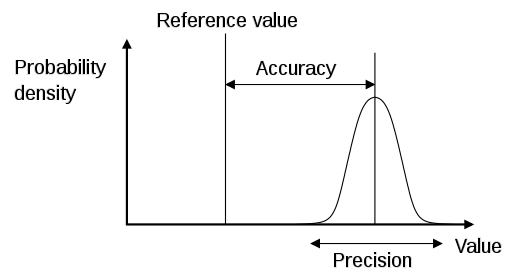
\includegraphics[height=2 in,clip]{../figs/accuracy-and-precision}
\end{center}
  \caption{"Accuracy and precision" by Pekaje at English Wikipedia - Transferred from en.wikipedia to Commons.. Licensed under GFDL via Commons - https://commons.wikimedia.org/wiki/File:Accuracy\_and\_precision.svg\#/media/
  File:Accuracy\_and\_precision.svg}
  \label{fig:accuracy}
\end{figure}
%
\textit{Accuracy} is the degree of closeness of measurements of a quantity to that quantity's true value.\\
The \textit{precision} of a measurement system, related to reproducibility and repeatability, is the degree to which repeated measurements under unchanged conditions show the same results.
% https://en.wikipedia.org/wiki/Accuracy_and_precision

Accuracy can be affected by systematic errors in simulation: physical and mathematical models; errors in geometry or source model; incorrect code use by user.\\
Usually unknown.

Conversely, precision can usually be improved: run more histories; use variance reduction; adjust your measurement (fewer scoring bins).

\vspace*{1 em}
%-------------------------------------------------------
-------------------------------------------------------\\
\textbf{Variance Reduction}\\
What we have talked about so far is \textit{Analog} Monte Carlo:
\begin{itemize}
    \item Natural laws are \textbf{preserved}
    \item The game is the ``analog" of the physical problem of interest (the history of each particle is simulated exactly)
    \item No alteration of PDFs
    \item At collision, particle is killed if absorption
    \item Particle is born with weight 1
    \item weight unchanged throughout history
    \item Score when tallying events is 1
\end{itemize}
%
We often, instead, want to do \textit{Non-Analog} Monte Carlo:
\begin{itemize}
    \item To reduce computation time, the strict analog simulation of particles is abandoned
    \item Variance Reduction techniques: Absorption suppression, Russian Roulette (history termination), Splitting (history propagation), Forced collisions, Source biasing, Hybrid methods
    \item Alter PDFs to favor events of interest
    \item Particle can have different birth weight
    \item Weight is altered if biased PDF is used
    \item Particle survives ``absorption" and weight is changed
    \item Splitting and RR can change weight
    \item Score current weight when tallying
\end{itemize}
%
We'll talk about implicit capture (a.k.a.\ survival biasing), roulette, splitting, and weight window maps. 

The first thing to think about is how to measure success. How do we know if a calculation is ``better"?\\
We use the figure of merit
\[
FOM =\frac{1}{R^2 t}\:,
\]
where $R$ is the relative error and $t$ is the particle tracking time.\\
What we really want is to reduce both of these. \\
Why are they related to one another this way? Recall that $S_x \propto \sqrt{\frac{1}{N}}$.\\
It's clear that without variance reduction techniques to reduce error by a factor of two you need to increase particle count (and hence time) by a factor of four.\\
FOM measures if we're really winning.

\textit{The idea of VR is to track particles that will contribute meaningfully to the desired results and to avoid tracking those that will not while maintaining a fair game.}

\end{document}
